\documentclass[conference]{IEEEtran}
\IEEEoverridecommandlockouts
\usepackage{cite}
\usepackage{amsmath}
\usepackage{graphicx}
\usepackage{booktabs}
\usepackage{array}
\usepackage[T1]{fontenc}
\usepackage{url}
\def\BibTeX{{\rm B\kern-.05em{\sc i\kern-.025em b}\kern-.08em
    T\kern-.1667em\lower.7ex\hbox{E}\kern-.125em X}}

\newcommand{\sig}[1]{\texttt{\detokenize{#1}}}
\newcommand{\sigp}[1]{{\ttfamily\path{#1}}}

\begin{document}

\title{Design and Performance Analysis of a Direct-Mapped Cache Controller Using Verilog}

\author{\IEEEauthorblockN{Priyal (2401010354), Anusha (2401010344), Kashika (2401010215),\\
Vaishnavi (2401010489), Sarthak (2401010420)}
\IEEEauthorblockA{\textit{Department of Computer Science and Engineering, Newton School of Technology}\\
Modern Computer Architecture --- Project 6}}

\maketitle

\begin{abstract}
This paper presents the design, register-transfer level (RTL) implementation, and performance evaluation of a direct-mapped cache controller in synthesizable Verilog, connected to a fixed-latency main-memory model. The controller manages a 1~KB level-one data cache divided into 64 lines of 16 bytes each. For a 32-bit byte address, the fields are split into a 22-bit tag, a 6-bit index, and a 4-bit block offset. We implemented a write-through policy that is no-write-allocate by default, which keeps the controller simple and main memory consistent, and added a \sig{WRITE_ALLOCATE} parameter that switches the controller to write-allocate. The datapath uses three storage structures: a 64-line by 4-word data RAM, a 64-entry tag RAM, and a 64-bit valid array that is cleared on reset. A 5-state finite-state machine (FSM) controls lookup, refill, and memory write cycles, and a busy output tells the processor when a request is in progress. We verified the design with both a self-checking testbench covering seven test groups and a trace-driven testbench running eight access traces. All tests passed with zero data errors. With a main-memory latency of 4 cycles, a hit takes 3 cycles and a read miss takes 23. The simulations showed hit rates of 75\% for sequential reads, 99.5\% for repeated loops, 23.9\% for random access, and 0\% for stride-16, stride-1024 and column-major matrix access, clearly demonstrating spatial locality, temporal locality, and conflict misses. Synthesis and further analysis are planned for Phase II.
\end{abstract}

\begin{IEEEkeywords}
Direct-Mapped Cache, Cache Controller, Verilog HDL, Finite State Machine, Memory Hierarchy, Trace-Driven Simulation, AMAT.
\end{IEEEkeywords}

%==============================================================
\section{Literature Review}

Processors have gotten much faster than DRAM. That gap --- called the memory wall --- is why caches exist. As clock frequencies scaled into the gigahertz range, off-chip memory access times failed to keep pace, leaving processors waiting for tens or hundreds of idle cycles during main-memory transfers. Fast on-chip SRAM caches bridge this speed difference by keeping recently used data near the CPU. Jhamb, Sharma, and Gupta \cite{jhamb} present a high-level VHDL implementation of an asynchronous, micropipelined Level-I cache on an FPGA, using direct-mapped, write-through data and instruction caches, and evaluate its performance. It is an example of a cache designed in a hardware description language and evaluated for performance, similar in spirit to our Verilog design.

Direct-mapped caches offer the simplest and fastest cache design. In a direct-mapped layout, every block in physical memory maps to exactly one specific line in the cache, determined by its address bits. This setup avoids the multi-input comparator trees and associative multiplexers needed by set-associative designs, making hit detection fast. Wang and Baer \cite{wang} developed efficient trace-driven simulation methods that evaluate cache performance, such as hit ratio, across many cache configurations from the same address trace. This motivates our own trace-driven evaluation. In our design, a 32-bit address is split directly into tag, index, and word offset fields, so hit detection requires only a single comparator check.

A cache works because programs exhibit locality of reference. Spatial locality means that when a program accesses one memory word, it will likely access nearby words soon after; temporal locality means that recently accessed data will likely be reused in the near future. Hassan et al.\ \cite{hassan} study synthetic trace-driven simulation of cache memory: generating synthetic memory traces that reflect locality, and using them to study cache performance under different workloads and configurations. In our verification setup, we use synthetic traces to stress-test sequential, repeated, strided, and matrix-based access patterns.

Despite their clock speed advantages, direct-mapped caches suffer from conflict misses. A conflict miss happens when two or more active memory blocks map to the exact same cache index, forcing one block to evict the other even when most of the cache sits empty. Jouppi \cite{jouppi} studied the limitations of direct-mapped caches, including conflict misses, and proposed adding a small fully-associative cache and prefetch buffers to reduce their cost. Jouppi's table of rising miss costs also shows why miss penalty matters for AMAT. In our work, we observe conflict behaviour directly: the stride-1024 trace (the stride equals the cache size, so every access maps to the same index) produces a 0\% hit rate, and the conflict test in our testbench also shows very low hit rates.

Hennessy and Patterson \cite{hp} classify cache write policies into two main families: write-through and write-back. In a write-through cache, every write updates both the cache and main memory immediately, keeping backing memory consistent at all times and removing the need for dirty bits or write-back buffers on eviction. On a write miss, the system can either fetch the missing block first (write-allocate) or send the write directly to memory without changing cache contents (no-write-allocate). In our design, choosing write-through with no-write-allocate as the default keeps the controller logic minimal and state transitions simple. Hennessy and Patterson \cite{hp} also define the standard formula for Average Memory Access Time (AMAT):
\begin{equation}
\text{AMAT} = \text{Hit Time} + (\text{Miss Rate} \times \text{Miss Penalty})
\end{equation}
This metric shows that overall memory performance depends not just on hit rate, but on the penalty paid during every refill. In hardware, miss penalty depends on the bus handshake and main-memory read latency.

Our MCA lecture notes \cite{notes} cover the memory hierarchy and caches. In our design, the controller must wait for a memory acknowledge for each word it transfers, so main-memory latency directly determines the miss penalty: with $\text{LAT}=4$, a hit takes 3 cycles and a read miss takes 23, a penalty of 20 cycles. When memory latency increases, the penalty of every miss grows, which makes the hit rate even more important.

The papers above cover cache hardware implementation \cite{jhamb}, trace-driven evaluation \cite{wang}, \cite{hassan} and the limits of direct-mapped caches \cite{jouppi}, but each addresses one part of the problem. We combine these parts in one small, open design: a synthesizable Verilog direct-mapped controller with a write-policy parameter, a self-checking testbench, a fault-injection check, and trace-driven performance measurement with AMAT, all in one repository.

%==============================================================
\section{Proposed Solution}

\subsection{System Architecture}
The developed system comprises a direct-mapped level-one (L1) data cache controller implemented in synthesizable Verilog, interfaced between an upstream processor/testbench interface and a downstream fixed-latency main-memory model. On the processor-facing side, the cache controller accepts four primary input signals: a single-bit request flag (\sig{req}), an active-high write-enable flag (\sig{we}), a 32-bit byte address (\sig{addr}), and 32-bit write data (\sig{wdata}). The controller responds with a 32-bit read data output (\sig{rdata}) and a single-cycle completion flag (\sig{done}). A busy status output tells the upstream CPU that a transaction is in progress, so it can avoid issuing requests mid-transaction. The controller also provides hit, miss, memory-read and memory-write counters (\sig{hits}, \sig{misses}, \sig{mem_reads}, \sig{mem_writes}).

On the memory-facing side, the cache controller interfaces with a main-memory module via a synchronous handshake channel. The controller issues a memory request (\sig{mem_req}), write-enable (\sig{mem_we}), memory word address (\sig{mem_addr}), and memory write data (\sig{mem_wdata}). The main-memory module acknowledges transactions using a memory acknowledge signal (\sig{mem_ack}) and delivers fetched words over a memory read data bus (\sig{mem_rdata}). The complete data path coordinates transaction flow as follows: CPU/Testbench feeds the cache controller, which arbitrates between the storage RAMs / tag comparator and the main-memory handshake, returning results to the CPU (see Fig.~\ref{fig:block}).

\begin{figure*}[!t]
\centering
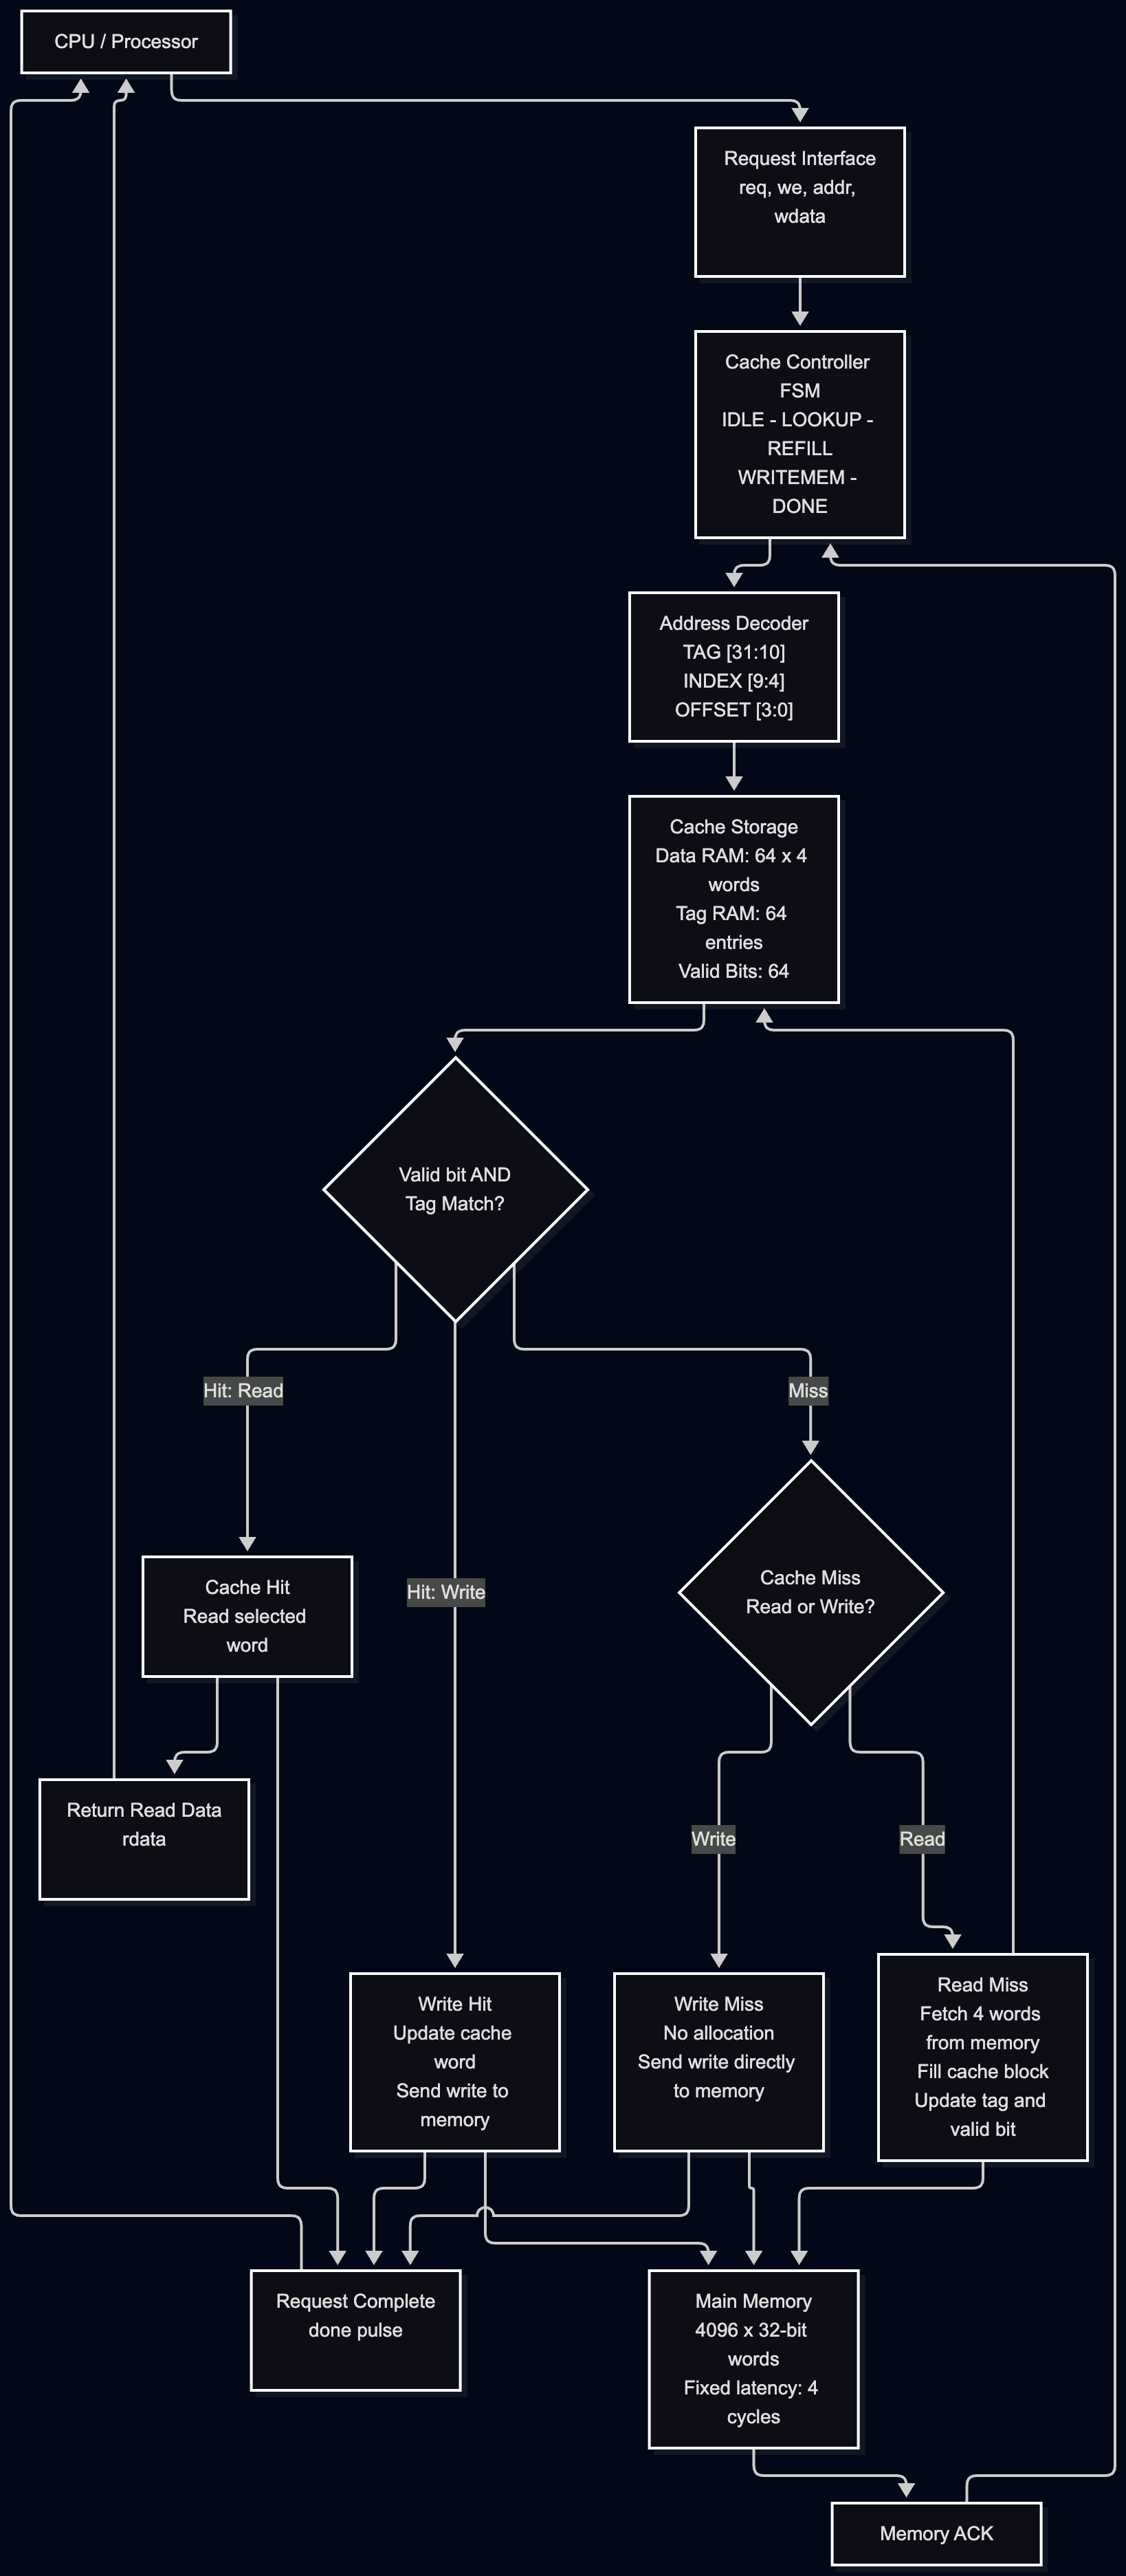
\includegraphics[angle=90,width=\textwidth]{block_diagram.png}
\caption{System block diagram of the direct-mapped cache controller and main-memory interface.}
\label{fig:block}
\end{figure*}

\subsection{Address Decomposition}
The cache controller operates on 32-bit byte addresses ($A = [31{:}0]$) referencing a 1~KB total data storage capacity organized into 16-byte cache blocks (lines). Address decomposition proceeds deterministically according to the physical parameters:
\begin{enumerate}
\item \textbf{Block Offset:} A 16-byte block contains four 32-bit words ($4 \times 4 = 16$ bytes). The byte offset requires $\log_2(16) = 4$ bits ([3:0]). Specifically, bits [1:0] address individual bytes within a 32-bit word, while bits [3:2] select the target word within the 4-word block.
\item \textbf{Index:} The total number of cache lines is determined by dividing total capacity by block size: Lines $= 1024\,\text{B} / 16\,\text{B} = 64$ lines. Indexing 64 lines requires $\log_2(64) = 6$ bits ([9:4]).
\item \textbf{Tag:} The remaining upper address bits form the tag identifier: Tag Width $= 32 - 6 - 4 = 22$ bits ([31:10]).
\end{enumerate}
The 32-bit address layout is structured as: [31:10] Tag field (22 bits), [9:4] Line Index field (6 bits), and [3:0] Block Offset field (4 bits). Internally, the storage architecture comprises three distinct arrays:
\begin{itemize}
\item \sig{data_ram}: Sized as 64 lines $\times$ 4 words (256 words of 32 bits each), addressed by concatenating the 6-bit index with the 2-bit word select: \sig{{idx, word_sel}}.
\item \sig{tag_ram}: An array of 64 entries, each storing a 22-bit tag associated with the resident cache line.
\item \sig{valid_ram}: An array of 64 single-bit registers indicating block residency. Crucially, the valid-bit array is synchronously cleared to zero upon system reset, guaranteeing that uninitialized SRAM contents cannot generate false cache hits.
\end{itemize}
Hit detection combines these three arrays combinationally:
\begin{equation*}
\texttt{hit} = \texttt{valid\_ram[idx]} \;\&\&\; (\texttt{tag\_ram[idx]} == \texttt{tag})
\end{equation*}

\subsection{Cache Controller FSM}
The operational control flow is governed by a five-state Finite State Machine (FSM):
\begin{enumerate}
\item \textbf{IDLE:} Default quiescent state. Both \sig{mem_req} and \sig{mem_we} remain deasserted (0), and the FSM monitors the input \sig{req} signal. Upon detecting \sig{req == 1}, the controller captures the address and data inputs and transitions to LOOKUP.
\item \textbf{LOOKUP:} The controller reads \sig{valid_ram[idx]} and \sig{tag_ram[idx]}, simultaneously comparing the stored tag against address bits [31:10]. On a read hit (\sig{!we && hit}), read data is routed directly to \sig{rdata} and the FSM transitions to DONE, where the single-cycle \sig{done} pulse is asserted. On a read miss (\sig{!we && !hit}), the controller initiates a line refill by asserting \sig{mem_req = 1}, \sig{mem_we = 0}, resetting an internal word refill counter, and transitioning to REFILL. On a write transaction (\sig{we}), the controller asserts \sig{mem_req = 1}, \sig{mem_we = 1}, and transitions to WRITEMEM (write-through). If the write is a hit, \sig{data_ram} is updated in parallel. With the optional \sig{WRITE_ALLOCATE} parameter set, a write miss instead goes to REFILL to fetch the line first, and then to WRITEMEM for the write.
\item \textbf{REFILL:} The controller performs a burst-like refill across four successive words. It asserts \sig{mem_req = 1} and issues sequential word addresses to main memory. Upon each assertion of \sig{mem_ack} by main memory, the incoming \sig{mem_rdata} is written to \sig{data_ram[{idx, counter}]}, and the counter increments. When the fourth word (\sig{counter == 3}) is acknowledged, the controller updates \sig{tag_ram[idx] <= tag}, sets \sig{valid_ram[idx] <= 1'b1}, deasserts \sig{mem_req}, and transitions to DONE (or to WRITEMEM when the refill was caused by a write miss under write-allocate).
\item \textbf{WRITEMEM:} The controller maintains \sig{mem_req = 1} and \sig{mem_we = 1} until the memory model asserts \sig{mem_ack}. Upon receiving \sig{mem_ack}, main memory write completion is verified, \sig{mem_req} is deasserted, and the FSM transitions to DONE.
\item \textbf{DONE:} The controller asserts the external single-cycle \sig{done} pulse, clears internal flags, and transitions unconditionally back to IDLE to accept subsequent requests.
\end{enumerate}
Fig.~\ref{fig:fsm} shows the complete state-transition diagram with output assertions per state.

\begin{figure}[!t]
\centering
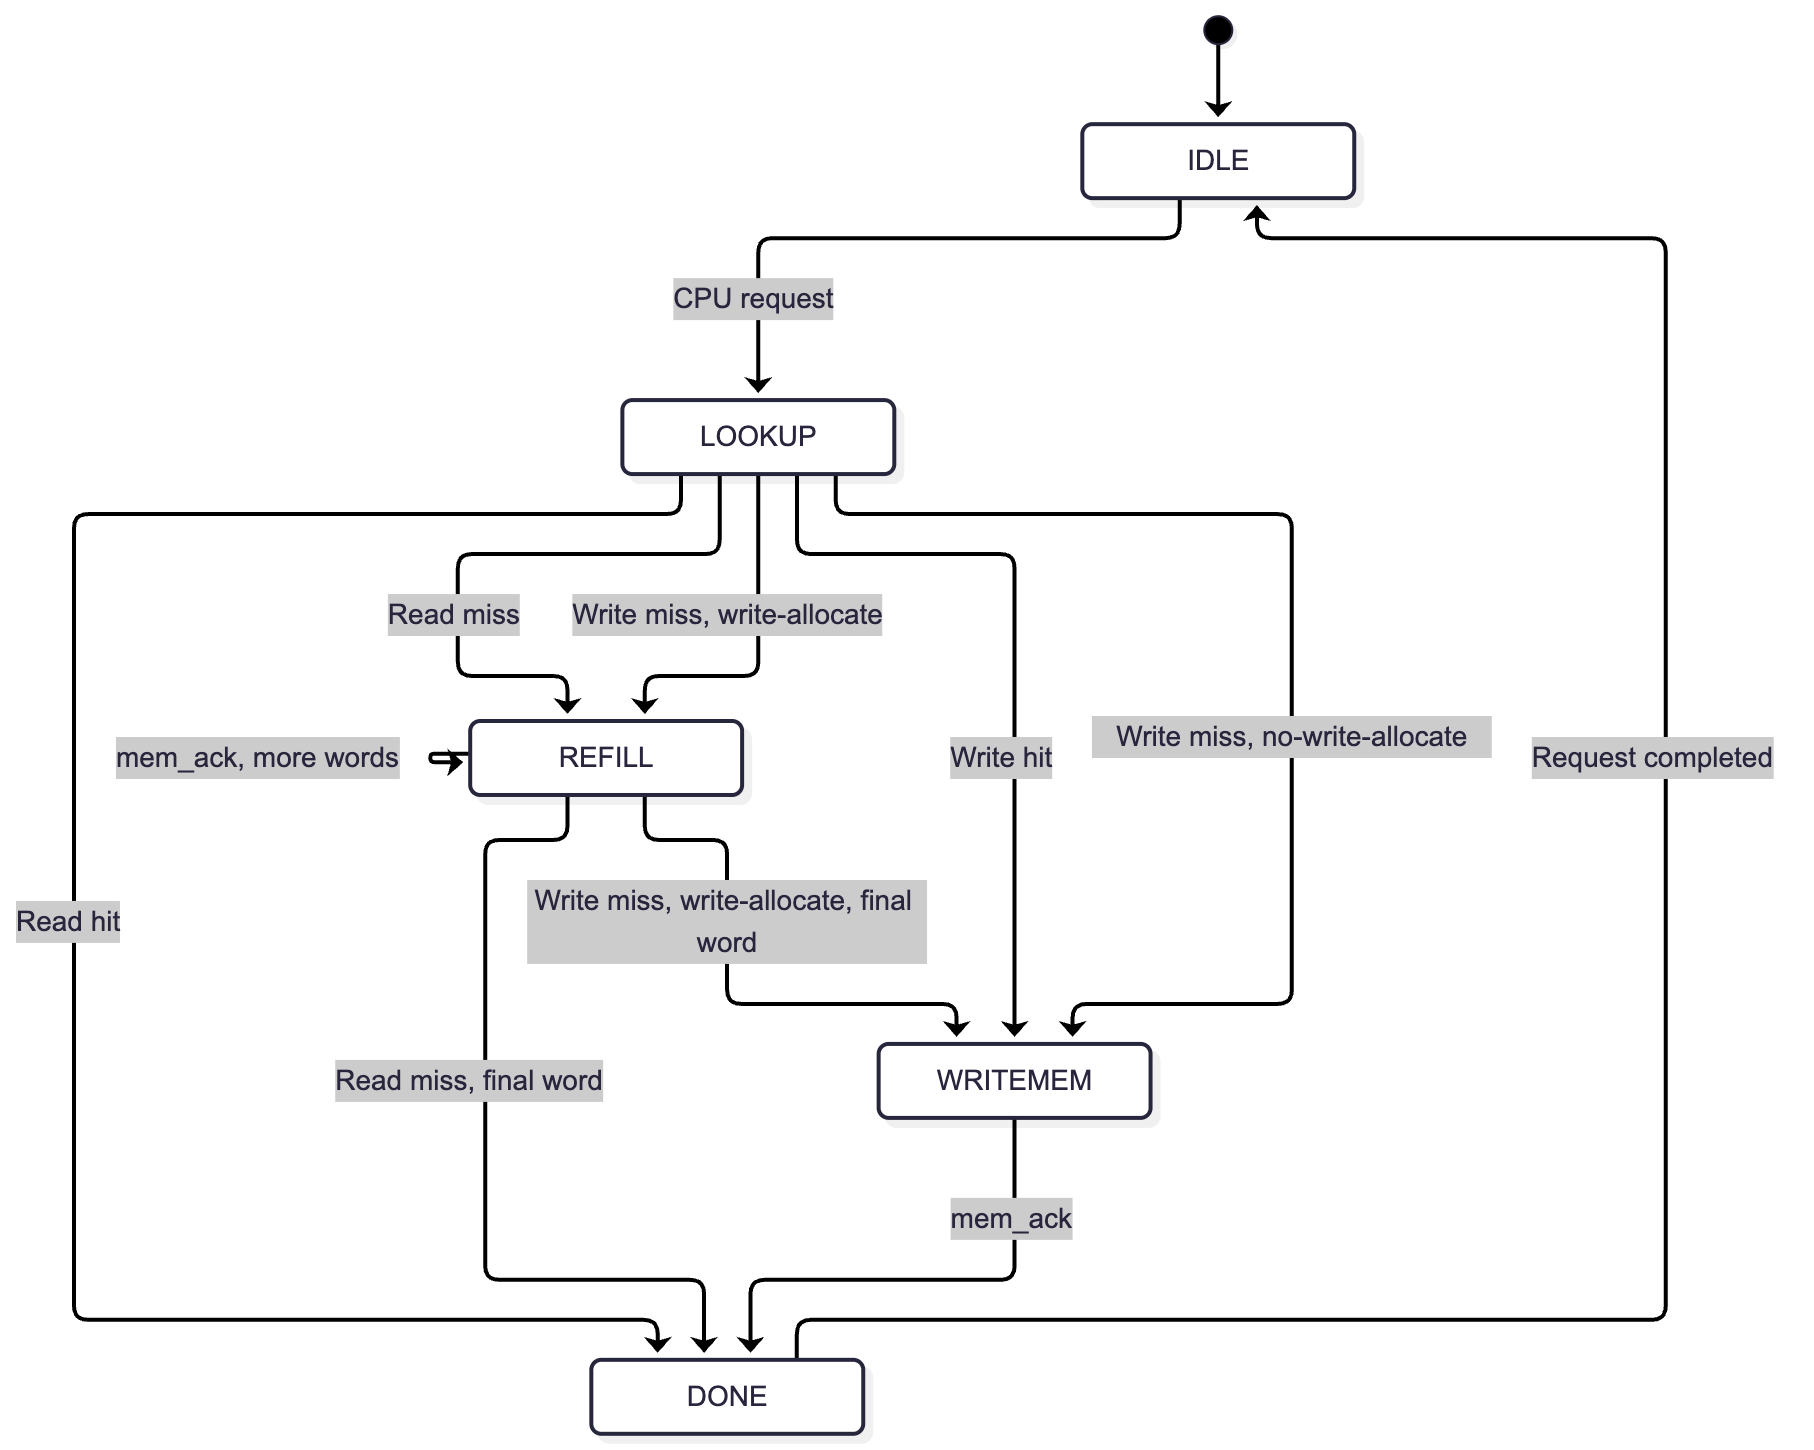
\includegraphics[width=\columnwidth]{fsm_diagram.png}
\caption{Controller FSM with per-state output assertions.}
\label{fig:fsm}
\end{figure}

\subsection{Module Hierarchy}
The project repository is structured modularly across functional hardware and verification directories:
\begin{itemize}
\item \sig{rtl/dm_cache.v}: Core parameterizable direct-mapped cache controller combining datapath registers, tag comparators, valid bits, and the 5-state FSM. Parameterized by \sig{INDEX_BITS} (default 6), \sig{WORD_BITS} (default 2) and \sig{WRITE_ALLOCATE} (default 0).
\item \sig{rtl/main_mem.v}: Word-addressed synchronous main-memory behavioral model implementing a configurable latency parameter \sig{LAT} (default 4 clock cycles) and a 4096-word (16~KB) memory (\sig{DEPTH} parameter), with explicit request-acknowledge handshaking.
\item \sig{tb/tb_dm_cache.v}: Directed, self-checking verification testbench executing corner-case functional test suites.
\item \sig{tb/tb_trace.v}: Trace-driven simulation engine accepting command-line runtime arguments (\sig{+TRACE=traces/<name>.trace}) to execute arbitrary access streams and record runtime metrics.
\item \sig{tb/tb_write_allocate.v}: Directed test of the optional write-allocate mode.
\item \sig{tb/tb_lat_sweep.v}: Runs the directed tests at memory latencies of 2, 4 and 8 cycles to measure the effect of latency on hit time, miss penalty and full line fill.
\item \sig{scripts/trace_gen.py}: Python automation utility generating synthetic memory traces formatted as hexadecimal read/write transactions (\sig{R/W <hex_addr> <hex_data>}).
\end{itemize}

\subsection{Write Policy}
The baseline implementation adopts a write-through with no-write-allocate policy. This configuration represents the most robust and hardware-efficient baseline for direct-mapped caches:
\begin{itemize}
\item Under write-through, every write transaction immediately propagates to main memory, ensuring that memory contains the latest data and eliminating the need for dirty bits or write-back flush sequences upon eviction.
\item Under no-write-allocate, write misses bypass the cache lines entirely, writing directly to main memory without evicting resident lines.
\item A write-allocate variant is implemented and selected with the \sig{WRITE_ALLOCATE} parameter (default 0). Under this policy, a write miss triggers a line refill from main memory before the written word is committed, which can improve hit rates for workloads with write-then-read temporal reuse. It is verified with \sig{tb/tb_write_allocate.v}. The default remains no-write-allocate.
\end{itemize}

\subsection{Verification Methodology}
We verified the design in two ways: a self-checking testbench with directed tests, and a trace-driven testbench with real workloads:
\begin{enumerate}
\item \textbf{Self-Checking Directed Testbench (\sig{tb_dm_cache.v}):} Maintains an internal golden reference memory array (\sig{ref_mem[]}). On every read transaction, the testbench compares the cache output \sig{rdata} against \sig{ref_mem[addr]}. Any discrepancy prints an explicit simulation ERROR and increments a failure counter. The directed suite executes seven test groups: first access after reset, repeated reads exercising temporal hit loops, conflict sequences accessing addresses separated by the cache capacity (1024 bytes), write hit with read-back, write miss with no-write-allocate, pseudo-random read sweeps across a 16~KB memory space, and filling all 64 lines. It also checks the busy output.
\item \textbf{Deliberate-Bug Fault Injection:} To ensure verification testbench rigor, a deliberate bug was injected into \sig{rtl/dm_cache.v} by removing the valid-bit comparison (\sig{hit = (tag_ram[idx] == tag)}). The self-checking testbench immediately caught the uninitialized RAM hits, reporting 275 failure errors and an immediate first-access mismatch, captured in \sigp{docs/results/valid_check_removal_275_failures.png} and \sigp{docs/results/valid_check_removal_first_access_error.png}.
\item \textbf{Trace-Driven Simulation (\sig{tb_trace.v}):} Evaluated eight memory access traces (sequential, random, repeated, stride-16, stride-1024, row-major matrix, column-major matrix and a write-intensive trace), generated by \sigp{scripts/trace_gen.py}, reporting total accesses, hits, misses, hit rate, miss rate, average execution cycles per access, AMAT, and no-cache baseline comparisons.
\item \textbf{Waveform Analysis:} Signal-level timing was analyzed in a waveform viewer (Surfer/WaveTrace) from captured Value Change Dump (\sig{dm_cache.vcd}) files, providing verified waveform evidence for read misses with 4-word refill handshakes, subsequent single-cycle read hits, and same-index conflict evictions.
\item \textbf{Latency Experiment (\sig{tb_lat_sweep.v}):} The directed tests were repeated at memory latencies of 2, 4 and 8 cycles. Filling a full line took 15, 23 and 39 cycles respectively, showing that main-memory latency directly sets the miss penalty.
\end{enumerate}

\subsection{Known Simplifications}
We deliberately kept the Phase I scope simple in four ways:
\begin{itemize}
\item Execution operates non-pipelined, processing a single memory request to full completion (\sig{done}) before accepting subsequent inputs.
\item The default write policy is write-through with no-write-allocate, trading memory write bandwidth for control simplicity.
\item The memory subsystem assumes a fixed response latency ($\text{LAT}=4$ cycles) without simulating multi-master bus contention or DRAM refresh stalls.
\item Verification sweeps constrain active address spaces to a 16~KB window, matching the 16~KB window modeled by \sig{main_mem.v}.
\end{itemize}

%==============================================================
\section{Individual Contributions}
The responsibilities and deliverables for Phase I were distributed among all five team members as summarized in Table~\ref{tab:contrib}.

\begin{table*}[!t]
\caption{Phase I Individual Contributions}
\label{tab:contrib}
\centering
\footnotesize
\renewcommand{\arraystretch}{1.15}
\begin{tabular}{|p{0.07\textwidth}|p{0.14\textwidth}|p{0.46\textwidth}|p{0.24\textwidth}|}
\hline
\textbf{Name} & \textbf{Role} & \textbf{Contribution (Phase I)} & \textbf{Files Owned}\\
\hline
Priyal & Cache Datapath, Performance \& Repo Lead & Address-field derivation; Data/Tag/Valid RAM + comparator; trace-driven testbench; hit/miss and AMAT results; baseline comparison; parameter sweep; created GitHub repo; wrote README and .gitignore; wrote Phase I video script & \sig{rtl/dm_cache.v} (datapath), \sig{tb/tb_trace.v}, README.md, .gitignore, results tables, sweep CSV\\
\hline
Anusha & Controller, Memory Interface \& Synthesis Lead & Cache controller FSM; main\_mem.v and handshake; write-allocate variant (WRITE\_ALLOCATE parameter and tb\_write\_allocate.v); busy output and memory-traffic counters; FSM diagram; LAT experiments (tb\_lat\_sweep.v) & \sig{rtl/dm_cache.v} (FSM), \sig{rtl/main_mem.v}, \sig{tb/tb_write_allocate.v}, \sig{tb/tb_lat_sweep.v}, \sig{docs/diagrams/fsm.md} and \sig{fsm_diagram.png}\\
\hline
Kashika & Verification Lead & Self-checking testbench; directed corner-case tests; annotated waveform screenshots; deliberate-bug check & \sig{tb/tb_dm_cache.v}, waveform screenshots in \sig{docs/waveforms/}, bug test screenshots in \sig{docs/results/}\\
\hline
Vaishnavi & Traces \& Plots Lead & Trace generator and trace files; system block diagram; plots from the results CSV; collected the literature review sources & \sig{scripts/trace_gen.py}, \sig{traces/}, plots, block diagram, source list\\
\hline
Sarthak & Report \& Demo Lead & Wrote the whole IEEE report (Abstract, Literature Review, Proposed Solution, Individual Contributions, References); assembled the Phase I video from the team's segments; submitted the submission form & \sigp{report/MCA_Project6_Report.pdf}, \sig{report/source/}\\
\hline
\end{tabular}
\end{table*}

%==============================================================
\begin{thebibliography}{00}
\bibitem{jhamb} M. Jhamb, R. K. Sharma, and A. K. Gupta, ``A High Level Implementation and Performance Evaluation of Level-I Asynchronous Cache on FPGA,'' \textit{Journal of King Saud University -- Computer and Information Sciences}, vol. 29, no. 3, pp. 410--425, 2017. \url{https://doi.org/10.1016/j.jksuci.2015.06.003}
\bibitem{wang} W.-H. Wang and J.-L. Baer, ``Efficient Trace-Driven Simulation Methods for Cache Performance Analysis,'' in \textit{Proc. ACM SIGMETRICS}, 1990, pp. 27--36. \url{https://doi.org/10.1145/98457.98497}
\bibitem{hassan} R. Hassan, A. Harris, N. Topham, and A. Efthymiou, ``Synthetic Trace-Driven Simulation of Cache Memory,'' in \textit{Proc. 21st Int. Conf. Advanced Information Networking and Applications Workshops}, 2007, pp. 764--771. \url{https://doi.org/10.1109/AINAW.2007.345}
\bibitem{jouppi} N. P. Jouppi, ``Improving Direct-Mapped Cache Performance by the Addition of a Small Fully-Associative Cache and Prefetch Buffers,'' in \textit{Proc. 17th Annual Int. Symp. Computer Architecture (ISCA)}, 1990, pp. 364--373. \url{https://doi.org/10.1145/325096.325162}
\bibitem{hp} J. L. Hennessy and D. A. Patterson, \textit{Computer Architecture: A Quantitative Approach}, 6th ed. Morgan Kaufmann, 2017.
\bibitem{notes} MCA Lecture Notes, Newton School of Technology (memory hierarchy and caches).
\end{thebibliography}

\end{document}